\documentclass[12pt]{article}

% Layout.
\usepackage[top=1in, bottom=0.75in, left=1in, right=1in, headheight=1in, headsep=6pt]{geometry}

% Fonts.
\usepackage{mathptmx}
\usepackage[scaled=0.86]{helvet}
\renewcommand{\emph}[1]{\textsf{\textbf{#1}}}

% TiKZ.
\usepackage{tikz, pgfplots}

\usetikzlibrary{calc,trees,positioning,arrows,fit,shapes,through, backgrounds}
\usetikzlibrary{patterns}

\usetikzlibrary{decorations.markings}
\usetikzlibrary{arrows}

\usepackage{pgfplots}


% Misc packages.
\usepackage{amsmath,amssymb,latexsym}
\usepackage{graphicx}
\usepackage{array}
\usepackage{xcolor}
\usepackage{multicol}
\usepackage{fancyhdr}
\pagestyle{fancy}


% Misc.
\renewcommand{\d}{\displaystyle}
\newcommand{\ds}{\displaystyle}
\newcommand{\ul}[1]{\underline{#1}}
\def\bc{\begin{center}}
\def\ec{\end{center}}
\def\be{\begin{enumerate}}
\def\ee{\end{enumerate}}

\newcommand{\ans}[1][1in]{\rule{#1}{.5pt}}


\lhead{Math F113X: Quiz 4}
\rhead{Feb 28, 2025}

\begin{document}

\vspace{1cm}
\strut

\noindent \textbf{Name:} \hrulefill \quad  score:\ans[1cm] \ / 10 \\


\noindent There are 10 points possible on this quiz. No aids (book, notes, etc.)
are permitted. You may use a calculator.  {\bf Show all work and supporting calculations for full credit. Explain how you get your answers.}



\be

\item (2 points) Describe a situation that can be modeled with a \emph{weighted} graph. What do the vertices represent? What do the edges represent? What do the weights represent?

Vertices:

\vfill

Edges: 

\vfill

Weights:

\vfill


\item (3 points) Consider the following graph:

\begin{center}
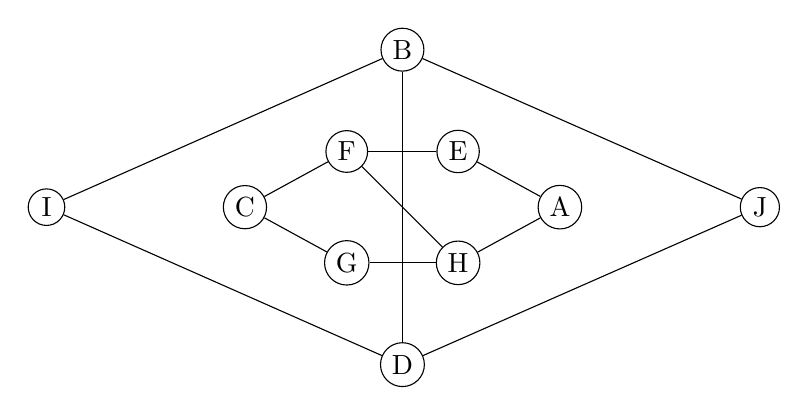
\begin{tikzpicture}[baseline=(current bounding box.center),]
\tikzstyle{vertex}=[circle, draw, inner sep=2pt]%, minimum size=6pt]

\tikzstyle{every node} = [vertex];
\node (A) at (0:2) {A};
\node (B) at (90:2) {B};
\node (C) at (180:2) {C};
\node (D) at (270:2) {D};
%\node (O) at (0,0){K};
\node (E) at (45:1) {E};
\node (F) at (45+90:1){F};
\node (G) at (45+180:1){G};
\node (H) at (45+270:1){H};
\node[left  = 2 cm of C] (I) {I};
\node [right = 2 cm of A] (J) {J};
\foreach \i/\j in {I/B,B/J,J/D, D/I,A/E,E/F,F/C,C/G,G/H,H/A,F/H, B/D}{\draw (\i) -- (\j);}
%\draw (B) -- (I) -- (D) -- (J)--(B);
%\draw (A) -- (E) -- (B) -- (F) -- (C) -- (G) -- (D) -- (H) -- (A);
%\draw (E) -- (O) -- (G) (F) --(O) --(H);
%\draw (A) -- (J) (C) -- (I);
%%\draw (I) to[looseness = 3, distance = 2in] (J);
%%\draw (I) to[looseness = 3, distance = -2in] (J);
%\draw (E) -- (F)  (G) -- (H);
\end{tikzpicture}
\end{center}

\be
\item How many vertices does this graph have? \ans
\item How many edges does this graph have? \ans
\item Explain why this graph is not connected.

\vspace{1in}
\ee

	\newpage
	
	\item (5 points) Recall Dijkstra's algorithm says the following:
	
	\fbox{Dijkstra's Algorithm}

\textbf{input:} a graph with distances (weights) on the edges and a starting vertex, say $s$\\
\textbf{output:} the shortest distance between $s$ and every vertex in the graph\\
\textbf{rough strategy:} All vertices get \emph{tentative} distances to vertex $s$. One-by-one, vertices are explored and tentative distances are updated until minimum distances are obtained. Break ties alphabetically.\\
%\textbf{Steps:}
%\begin{enumerate}
%	\item (Initialization Step) Set the tentative distance to be zero for $s$ and $\infty$ for all other vertices.
%	\item (Iterative Step) Find the vertex, say $x$, with the smallest tentative distance \textit{that has not already been explored}. (Break any ties alphabetically.)
%		\begin{enumerate} 
%		\item For every edge between $x$ and a vertex (say $y$) \textit{that has not already been explored}, calculate the sum of the distance to $x$ plus the distance along the edge to $y.$ If this sum is \emph{smaller} than the tentative distance at $y$, replace the tentative distance with the smaller value. Otherwise, leave the tentative distance of $y$ unchanged.
%		\item Mark $x$ as \emph{explored} and record its tentative distance to $s$ as its \emph{minimum} distance to $s.$
%		\item If $x$ is the last vertex then terminate the algorithm, otherwise return to the beginning of the iterative step.
%		\end{enumerate} 
%\end{enumerate}

	
	
	Use Dijkstra's algorithm to determine the distances between vertex $S$ and each other vertex. Clearly show the steps of the algorithm in the space provided.
	
	\begin{center}
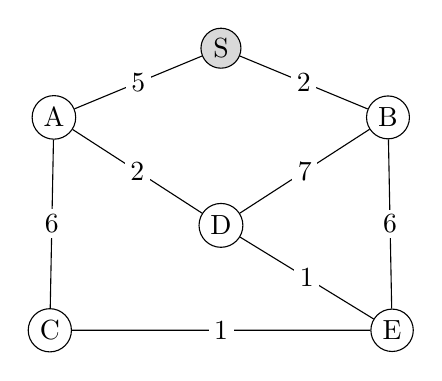
\begin{tikzpicture}[baseline=(current bounding box.center),lbl/.style={inner sep = 2pt, fill = white}, scale = 1.5]
\tikzstyle{vtx}=[circle, draw, inner sep=2pt]
\node[vtx, fill = gray!30] (S) at (90:2) {S};
\node[vtx] (A) at (135:2) {A};
\node[vtx] (B) at (45:2) {B};
\node[vtx] (D) at (90:0.5){D};
\node[vtx] (C) at (15+180:1.5){C};
\node[vtx] (E) at (-15:1.5){E};
\foreach \i/\j/\k in {S/A/5,S/B/2,A/C/6, A/D/2,B/D/7,B/E/6,C/E/1,E/D/1}{\draw (\i) --node[lbl]{\k} (\j);}
\end{tikzpicture}
\end{center}
\begin{minipage}[t]{.6\linewidth}
\begin{tabular}{ c | c | p{1.5in}}
Explored? & vertices & tentative distances\\ \hline
&S& \\[12pt] \hline
&A& \\[12pt]\hline
&B& \\[12pt]\hline
&C& \\[12pt]\hline
&D& \\[12pt]\hline
&E& \\[12pt]\hline
 \end{tabular}

 \end{minipage}
% 
\vspace{1cm}
%
 %
 \begin{minipage}{.4\linewidth}
 \begin{tabular}{ c | p{.8in} }
 vertex & minimum distance to S\\ \hline
S& \\[12pt] \hline
A& \\[12pt]\hline
B& \\[12pt]\hline
C& \\[12pt]\hline
D& \\[12pt]\hline
E& \\[12pt]\hline \end{tabular}
 \end{minipage}
\vfill


 \ee
\end{document}